\documentclass[12pt]{article}
\topmargin= -0.4in
\textheight = +8.9in
\oddsidemargin = 0.05in
\evensidemargin = 0.05in
\textwidth = 6.5in
\usepackage{times}
%\usepackage{babel}
\usepackage[capposition=top]{floatrow}
\usepackage{algpseudocode}
\usepackage{graphicx}
\usepackage{bm}
\usepackage[T1]{fontenc}
\usepackage[flushleft]{threeparttable}
\usepackage{lmodern}
\usepackage{graphicx}
\usepackage{amssymb,amsmath}
\usepackage{ifxetex,ifluatex}
\usepackage{fixltx2e} % provides \textsubscript
% use upquote if available, for straight quotes in verbatim environments
\IfFileExists{upquote.sty}{\usepackage{upquote}}{}
\ifnum 0\ifxetex 1\fi\ifluatex 1\fi=0 % if pdftex
  \usepackage[utf8]{inputenc}
\else % if luatex or xelatex
  \ifxetex
    \usepackage{mathspec}
    \usepackage{xltxtra,xunicode}
  \else
    \usepackage{fontspec}
  \fi
  \defaultfontfeatures{Mapping=tex-text,Scale=MatchLowercase}
  \newcommand{\euro}{€}
\fi
% use microtype if available
\IfFileExists{microtype.sty}{\usepackage{microtype}}{}
\usepackage{longtable,booktabs}
\ifxetex
  \usepackage[setpagesize=false, % page size defined by xetex
              unicode=false, % unicode breaks when used with xetex
              xetex]{hyperref}
\else
  \usepackage[unicode=true]{hyperref}
\fi
\hypersetup{breaklinks=true,
            bookmarks=true,
            pdfauthor={},
            pdftitle={},
            colorlinks=true,
            citecolor=blue,
            urlcolor=blue,
            linkcolor=black,
            pdfborder={0 0 0}}
\urlstyle{same}  % don't use monospace font for urls
\setlength{\parindent}{0pt}
\setlength{\parskip}{6pt plus 2pt minus 1pt}
\setlength{\emergencystretch}{3em}  % prevent overfull lines
\setcounter{secnumdepth}{0}

% Alter some LaTeX defaults for better treatment of figures:
    % See p.105 of "TeX Unbound" for suggested values.
    % See pp. 199-200 of Lamport's "LaTeX" book for details.
    %   General parameters, for ALL pages:
    \renewcommand{\topfraction}{0.9}	% max fraction of floats at top
    \renewcommand{\bottomfraction}{0.8}	% max fraction of floats at bottom
    %   Parameters for TEXT pages (not float pages):
    \setcounter{topnumber}{2}
    \setcounter{bottomnumber}{2}
    \setcounter{totalnumber}{4}     % 2 may work better
    \setcounter{dbltopnumber}{2}    % for 2-column pages
    \renewcommand{\dbltopfraction}{0.9}	% fit big float above 2-col. text
    \renewcommand{\textfraction}{0.07}	% allow minimal text w. figs
    %   Parameters for FLOAT pages (not text pages):
    \renewcommand{\floatpagefraction}{0.7}	% require fuller float pages
	% N.B.: floatpagefraction MUST be less than topfraction !!
    \renewcommand{\dblfloatpagefraction}{0.7}	% require fuller float pages

	% remember to use [htp] or [htpb] for placement








%\DeclareMathOperator*{\argmin}{arg\,min}

\begin{document}

\noindent
\thispagestyle{empty}
\underline{\bf Master's Paper of the Department of Statistics, the
  University of Chicago} 


\vspace{1.8in}
\begin{center}
{\bf\LARGE Combining Latent
Topics with Document Attributes in Text Analysis} \\~\\
%{A parallelizeable, computationally-minded approach } %Let's stew on this one...
%\\~\\
%{\bf\Large --- A Sample Format}


\vspace{1.4in}
{\Large Nelson Auner}

\vspace{1.3in}
{\Large Advisors: Prof. Matt Taddy\footnote{Associate Professor of Econometrics and Statistics at Chicago Booth School of Business}, Prof. Stephen Stigler\footnote{Ernest DeWitt Burton Distinguished Service Professor at the Department of Statistics of the University of Chicago} \\{\small }}

\end{center}

\vspace{.6in}
{\Large Approved} ~\underline{~~~~~~~~~~~~~~~~~~~~~~~~~~~~~~~~~~~~~~~~~~~~~~
~~~~~~~~~~~~~~~~~~~~~~~~~~~~~~~~~}

\vspace{.2in}
{\Large Date} ~~~~~~~~~\underline{~~~~~~~~~~~~~~~~~~~~~~~~~~~~~~~~~~~~~~~~~~~~~
~~~~~~~~~~~~~~~~~~~~~~~~~~~~~~~~~~~}


\newpage
\pagestyle{plain}
\setcounter{page}{1}

\begin{abstract}

\vspace{7mm}\noindent 

This paper introduces a variant to existing models of multinomial
regression for text analysis. Using the base model introduced by Taddy
(2013a), we extend the data-generating model to incorporate topics not
explained by metadata. In doing so, we seek to increase
the prediction accuracy over existing techniques, bridge the gap between
multinomial regression and standard topic models, and investigate
methods for discovering new topics in a corpus. We explore computational
aspects of our approach, provide software for parallelization of the
algorithm, and conclude by proposing areas of future research.

\end{abstract}

%\newpage
\vspace{1.5in}
\tableofcontents


\newpage


\section{Introduction}

\subsection{Motivation}


The analysis of data contained in natural language text is referred to as text mining or text analysis. 
The field has grown rapidly in popularity since the seminal 1963 paper (Mosteller and Wallace, 1663) that analyzed the
word usage patterns of James Madison and Alexander Hamilton to determine the authorship of disputed federalist papers.
More recently, through the advent of inexpensive computation and increasingly accessible digital information, widespread applications for text analysis have been developed in automated advertisement placement, business intelligence, finance, and national security. Among many examples are the use of text mining by drug companies to scan medical publications for promising drugs, and thus reduce R\&D costs (Belsky, 2012), and  an algorithm that measures political sentiment on twitter (Taddy, 2013c) which highlighted that GOP candidates are disproportionately the target of disparaging tweets. 

\subsection{Modeling Text Data}

%
\includegraphics{chick}

A common technique for modeling text data is the use of multinomial models on word `stems' derived from the original document.
Typically, text information is naturally grouped by documents, and each
document is represented by counts of words, or `tokens'. A document might be a
single written text (e.g.~an academic article), or a collection of works
by the same author (e.g.~all of the lyrics of an album by the Rolling
Stones) A token is often a single word (called a unigram) but may also be
a sequence of two or more words (e.g.`good swimmer' is a
bigram, and `I eat cheese' is a tri-gram). The word components of
tokens are often reduced to`stem' form by removing suffixes (e.g.
`illuminated', `illumination' and `illuminating' all become
`illuminate'), using the popular Porter stemming algorithm (Porter, 1980).

Since the number of unique words that appear in a large number of
documents can be extensive, we often restrict the number of tracked
tokens, $p$, to words or phrases that occur in at least two documents. If the total number of documents $n$ is large, we may also
remove common tokens that add little meaning and are found in almost all
documents (i.e. `the' or `of').

A trivial example of such content might be student's answers to the
question `What did homework assignments involve?', with the following four responses:

\begin{table}[!hbpt]
\caption{Example of text data from course reviews} \label{tab:title}
\begin{center}
\begin{tabular} {c c}
\textbf{Document} & \textbf{Content} \\
\hline
1 & Some computation and formula proving, a lot of R code \\
2 & Problems, computation using R \\
3 & Some computations and writing R code\\
4 & Proofs, problems, and programming work \\
\end{tabular}
\end{center}
\end{table}

These tokens are then aggregated by document: For $i$ in $1,...,n$,
the vector $x_i = [x_{i1}, x_{i2}, ... , x_{ip}]$ contains the
number of occurrences of first, second, \ldots{} $p$ th token in the
$i$th document, where $p$ is the total number of unique tokens in all
documents. This forms the complete count matrix $X = [x_1, x_2,..., x_n]^{T}$, where each $x_{ij}$
is the number of occurrences of word $j$ in document $i$.


Continuing with the example in Table 1 by removing common words and stemming the remaining words produces the count matrix $X$ in Table 2. 

\begin{table}[!hbpt]
\caption{Creating a word-count matrix from text}
\begin{center}
\resizebox{\textwidth}{!}{%
\begin{tabular}{ c |  c c c c c c c c c c c}
\hline
\textbf{Document} & Some & comp & formula & prov & R & code & use &
problem & writ & program & work \\
1 & 1 & 1 & 1 & 1 & 1 & 1 & 0 & 0 & 0 & 0 & 0 \\
2 & 0 & 1 & 0 & 0 & 1 & 0 & 1 & 1 & 0 & 0 & 0 \\
3 & 1 & 1 & 0 & 0 & 1 & 0 & 0 & 0 & 1 & 0 & 0\\
4 & 0 & 0 & 0 & 1 & 0 & 0 & 0 & 1 & 0 & 1 & 1\\
\hline
\end{tabular}}
\end{center}
\end{table} 



\subsection{Multinomial Model}\label{multinomial-model}

We then model each document $x_i$ as the realization of a multinomial
distribution. That is,

\[ x_{i} \sim MN(q_i,m_i) \]

where $q_i$ is the vector $[q_{i1}, \dots q_{ip}]$ of token
probabilities for document $x_i$ and $m_i$ is
$\sum_{j = 1}^{p}{x_{ij}}$, or the total number of tokens in document
$i$

It is trivial to show that the maximum likelihood estimator of $q_i$ is
$f_i$ = $x_i / m_i$, but by imposing structure on $q_i$, we can model
features of the data. The two most common techniques for creating
structure are \emph{topic models} and \emph{metadata}.

\subsection{Topic Models}\label{topic-models}

Under a topic model, each document is the realization of a
linear combination of $K$ topics, where each topic $l = 1,..,K$ represents a
distribution, or vector of probability weights
$\omega_l = [\omega_{l1}, ... , \omega_{lp}]$, over words. As a simple
example, we can imagine a fitness store that primarily sells books on
biking, running, and swimming. We can see that a probability
distribution of these topics would have high probability weights on the
terms (`pedal', `helment') for biking, (`stride') for running, and
(`breath', `stroke', `water') for swimming. By denoting the
proportion of topic $l$ as $\theta_l$, we can imagine each document as
being generated by a linear combination of topics
$\theta_1 \omega_1  + \theta_2 \omega_2 + \theta_3 \omega_3 $, described
as the following data-generating process:


\begin{enumerate}
\item 
Choose the number of words N 
\item
  Choose $\theta = \theta_1,...,\theta_K$, the proportion of topics.
  (i.e., a book completely about swimming would have $\theta=(1,0,0)$ ,
  a book about triathalons might have $\theta =(1/3,1/3,1/3)$ ).
\item
  For each word $w_i$:
\begin{enumerate}
\item Choose topic $l$ with probability $\theta_l$
\item
Choose  a word $w_{i}$ with the topic word-weighting vector $\omega_l$
\end{enumerate}
\end{enumerate}

Traditionally, the topic model proportions are given a Dirchlet prior, and the model is also known as Latent Dirichlet Allocation, or LDA. 
For a thorough introduction to topic models, we refer the reader to Blei, Ng, and Jordan (2003). 

\subsection{Metadata}\label{metadata}

Text data is frequently accompanied by information, or metadata, about
the text itself. For example, metadata on an academic
article could include the number of times the article has been cited,
and the journal in which the article has been published. We then seek to model the relationship between metadata
and the composition of the text. For example, given a database of
written movie reviews and final rating out of five $y \in (1,2,3,4,5)$,
we might want to predict the movie rating from the text content of the review.

\subsection{Metadata and Unigram Models}

If the support $Y$ of metadata $y$ takes discrete values $y^{(1)}, y^{(2)}, \dots, y^{(m)}$ with few unique observations ($m$ small), we can `collapse' the token counts over levels of metadata for simplification and computational gains.  That is, each dataset of $n$ ordered (text, metadata) pairs

\begin{equation}
\big[ (x_1,y_1), (x_2,y_2), \dots , (x_n,y_n) \big]
\end{equation}

can be expressed, as $m$ collapsed observations:

\begin{equation}
\big[  (\sum_{x_i : y_i = y^{(1)}}{x_i}) , (\sum_{x_i : y_i = y^{(2)}}{x_i}), \dots,  (\sum_{x_i : y_i = y^{(m)}}{x_i})  \big]
\end{equation}

Then, a simple log-link model allows us to express document $x$ with given metadata rating $y$,
denoted $x_y$, as $x_y \sim MN(q_y,m_y)$, with
\begin{equation}
q_{yj} \sim \frac{exp[\alpha_j + y \phi_j]}{\sum_{l=1}^{p} exp[\alpha_l + y \phi_l]}
\end{equation}

The coefficient $\phi$ is referred to as the \textit{distortion vector}. Intuitively, it \textit{distorts} the base frequency of words $\alpha$ by the effect of the metadata $y$. 
For example, if we had text information on college course evaluations written by students, and metadata of a value, from one to ten, representing the student's evaluation of the class, we would expect the distortion vector $\phi$ to have high loadings, or coefficients, on terms such as `interesting', `engaging', and `useful', and low loadings on the words `difficult', `boring' and `sleepy'. 

\section{Theory and Approach}\label{theory-and-approach}

\subsection{Mixture models and cluster
membership}\label{mixture-models-and-cluster-membership}

We now turn our attention to the main purpose of this paper, which is to
incorporate latent topics across documents while maintaining the computational simplicity of a collapsable multinomial model. To do so we will restrict our model by assuming that every document is a member of one and only one topic. In order not to confuse our approach with traditional topic models, where each topic can take a weight $\theta \in (0,1)$, we refer to the model in which a document can only belong to one topic as a \textit{cluster membership model}. This terminology also emphasizes the theoretical relationship between our model and finite mixture models, where every data point is generated by a specific mixture component.

As a simple motivating example, we might imagine a corpus of
movie reviews written by several bloggers. After accounting for text
information explained by the rating (e.g. ~relating a 5-star rating to
`good plot'), the remaining heterogeneity in the movie review
content could be related traits of the blogger (e.g.~gender, or home
city). We may be interested in predicting traits of bloggers
given their movie reviews, and also in determining how movie review
content changes across these traits. For example, we could examine how movie reviews written by 
female bloggers differ from movie reviews written by male bloggers.




\subsection{Model Specification}\label{model-specification}

Denoting the word count of a document as the vector $x_i$, we propose
that words in a document are distributed as a multinomial with a
log-link to document metadata and cluster membership. That is:

\begin{equation}
 x_{i} \sim MN(q_{ij},m_{ij})    ; ~~  q_{ij} = \frac{exp(\alpha_j + y_i \phi_j + u_i \Gamma_{kj})}{\sum_{l=1}^{p}{exp(\alpha_l+ y_i \phi_l + u_i \Gamma_{kl})}}
\end{equation} 


In our notation, $y_i$ and $u_i$ are the metadata and cluster membership associated
with document $i$. $u_i$ is an $n \times 1$ vector, and $y_i$ is a $n  \times N_m$ matrix, where $N_m$ is the number of metadata variables. $\alpha$ is the vector that correspond to a baseline or intercept of word frequencies. 
Using the same terminology introduced earlier, the coefficients $\phi_j$ and $\Gamma_{kj}$ are the distortion
vectors for metadata and cluster membership, respectively.

 We use
the subscript $k$ for cluster membership to denote that each document $x_i$ is considered a
member of one of $k = 1,..,K$ clusters, with their own distortion vectors
$\Gamma_1,..,\Gamma_K$

By collapsing over metadata, we can express the the distribution of a document $x$ given metadata $y$, $x_{yk}$, with

\begin{equation}
 x_{yk} \sim MN(q_{yk},m_{yk}), ~ ~ q_{yk} = \sum\limits_{i: y_i = y, u_i = k} \big[\sum_{j = 1}^{p} {x_{ij}} \big]
\end{equation}
and 
\begin{equation}
q_{yk} \sim \frac{exp[\alpha + y \phi  + u_k \Gamma_{k}]}{\sum_{l=1}^{p} exp[\alpha_j + y \phi_j+ u_k \Gamma_{kj} ]}
\end{equation}

\subsection{Estimation of Parameters via Maximum a
Posteriori}\label{estimation-of-parameters-via-maximum-a-posteriori}

The negative log likelihood of a multinomial distribution can be written
as

\begin{equation} 
\ell(\alpha,\phi,\Gamma,u) = \sum_{i = 1}^{N}{ x_i^\top (\alpha + \phi v_i + u_i \Gamma_{kj})} - m_i log(\sum_{j = 1}^{p}{exp{\big[ \alpha + \phi v_i + u_i \Gamma_{kj} \big]}})
\end{equation}

Following previous literature on text regression (Taddy 2013a), we specify Laplace priors and a gamma hyperprior on coefficients, as well as a gamma lasso penalty on coefficients $\Phi$ and $\Gamma)$. This
procedure leads us to minimize the sum of log likehood with the gamma lasso penalty.

\begin{equation}
\ell(\alpha,\Phi,\Gamma,u) = \sum_{j=1}^{p}(\alpha_j/ \sigma_\alpha)^2 + c(\Phi,\Gamma) 
\end{equation}


The procedure to fit the coeffecients of a multinomial with gamma lasso penalty are documented in Taddy (2013b). We now briefly detail the fitting of the cluster membership via Bayesian estimation:

\begin{equation}
\boldsymbol{u}^{*}_{MAP}  = \underset{\mathbf{u}}{\arg\max} \, \, \, P( \mathbf{u} | X) \\
\end{equation}
\begin{equation}
= \underset{\mathbf{u}}{\arg\max} \, \, \frac{P( \mathbf{u} | X) \, P(\boldsymbol{u})}{P(X)}    \\
\end{equation}
\begin{equation}
= \underset{\mathbf{u}}{\arg\max} P( \mathbf{u} | X) \, P(\boldsymbol{u})  \\
\end{equation}

And under the assumption that the $P(u_i) = P(u_j)$ for any two cluster vectors $u_i$, $u_j$, we eliminate $P(\boldsymbol{u})$:

\begin{equation}
\boldsymbol{u}^{*}_{MAP} = \underset{\mathbf{u}}{\arg\max} P( \mathbf{u} | X)
\end{equation}


Although the likelihood function cannot be solved analytically, the discrete support for \textbf{u} makes it trivial to check the entire parameter space.


 The algorithm we use to fit coefficients $\alpha$, $\phi$, $\Gamma$
and cluster memberships $u_i$ is two main steps iterated until
convergence:

\textbf{Algorithm for Cluster Membership Model with Gamma Lasso Penalty}
\begin{enumerate}
\def\labelenumi{\arabic{enumi}.}
\item
 Initialize $u_i$ for $i = 1, \dots, n$
\item
  Determine parameters $\alpha_, \phi, \Gamma$ by fitting a multinomial
  regression on $y_i | x_i , u_i$ with a gamma lasso penalty
\item
  For each document $i$, determine new cluster $u_i$ membership as \\
  $argmax_{k = 1,..,K} \big[  \ell(u_i| \alpha, \phi, \Gamma) \big]$
\item 
Check if current cluster assignment is different from previous cluster assignment, ($\textbf{u}^{(t)}  = \textbf{u}^{(t-1)}$). If so, return to step 2. If not, end algorithm.
\end{enumerate}


By alternating between the first two steps, we aim to converge to optimal
parameter estimates $\alpha, \phi, \Gamma$ as well as optimal cluster
memberships \textbf{u}.

In practice, the algorithm converged after less than 20 iterations for all three datasets that we tested, with between 5 and 20 clusters. To address possible issues of cycling or non-convergence, an option for a maximum number of iterations was included in the code. 
If the algorithm does not converge within the maximum number of iterations, the program would stop and return the current parameter estimates, as well as  notifying the user of non-convergence.

\subsection{Computation}\label{computation}
As noted previously, a property of multinomial regression is the ability to
collapse observations across levels of metadata without losing information. This attractive
property is preserved in the cluster membership model.

In step (2) of the algorithm, we can increase the speed by only evaluating portions of the likelihood function relevant to $u_i$ and $\Gamma_kj$ by eliminating first two terms from the full likelihood and penalty equation.

\begin{equation} 
\ell(u_i|\alpha,\phi,\Gamma) = \sum_{i = 1}^{N}{ x_i^\top (u_i \Gamma_{kj})} - m_i log(\sum_{j = 1}^{p}{exp{\big[ \alpha + \phi v_i + u_i \Gamma_{kj} \big]}})
\end{equation}

In addition, the rightmost term does not depend on $x_i$ and can be precalculated for each cluster $u_i$. This will lead to an order-of-magnitude speed-up as long as the number of clusters is relatively small compared to the number of documents. 


\subsection{Initializing Cluster Membership}

We begin our algorithm by initializating \textbf{u}, that is, assigning each document $u_i$ to a cluster. 
Because each document can only be a member of one topic (unlike a traditional topic model), we want to investigate how important the cluster member initialization is to the final coefficients. 
For this paper, we initialize cluster membership using one of the three following
methods:

\begin{enumerate}
\def\labelenumi{\arabic{enumi}.}
\itemsep1pt\parskip0pt\parsep0pt
\item
  Random Initialization
\item
  K-means on the word count data $X$
\item
  K-means on the residual of the word count data after incorporating
  metadata $y$ (that is, given predicted word count $\hat{X}$,
  clustering on $X-\hat{X}$
\end{enumerate}


\section{Application and Evaluation of Algorithm}\label{application}

We applied the Cluster Membership model to two datasets: Congressional Speech records, most famously used to investigate media slant (Gentzkow and Shapiro, 2010) and a corpus of restaurant reviews collected by the website we8there.

\subsection{Congressional Speech} 

We first investigate the performance of the algorithm on the congressional speech data. The data consists of text from 579 speeches of the members of the 109th Congress. For the analysis, party membership was regressed onto speech data. The algorithm was run for 5, 10, 15, 20, and 25 clusters, each over the 3 different initialization methods described in the previous section. We then report the multinomial deviance, or two times the negative log likelihood, in figure 1. 

\begin{figure}[!htpb]
  \centering
  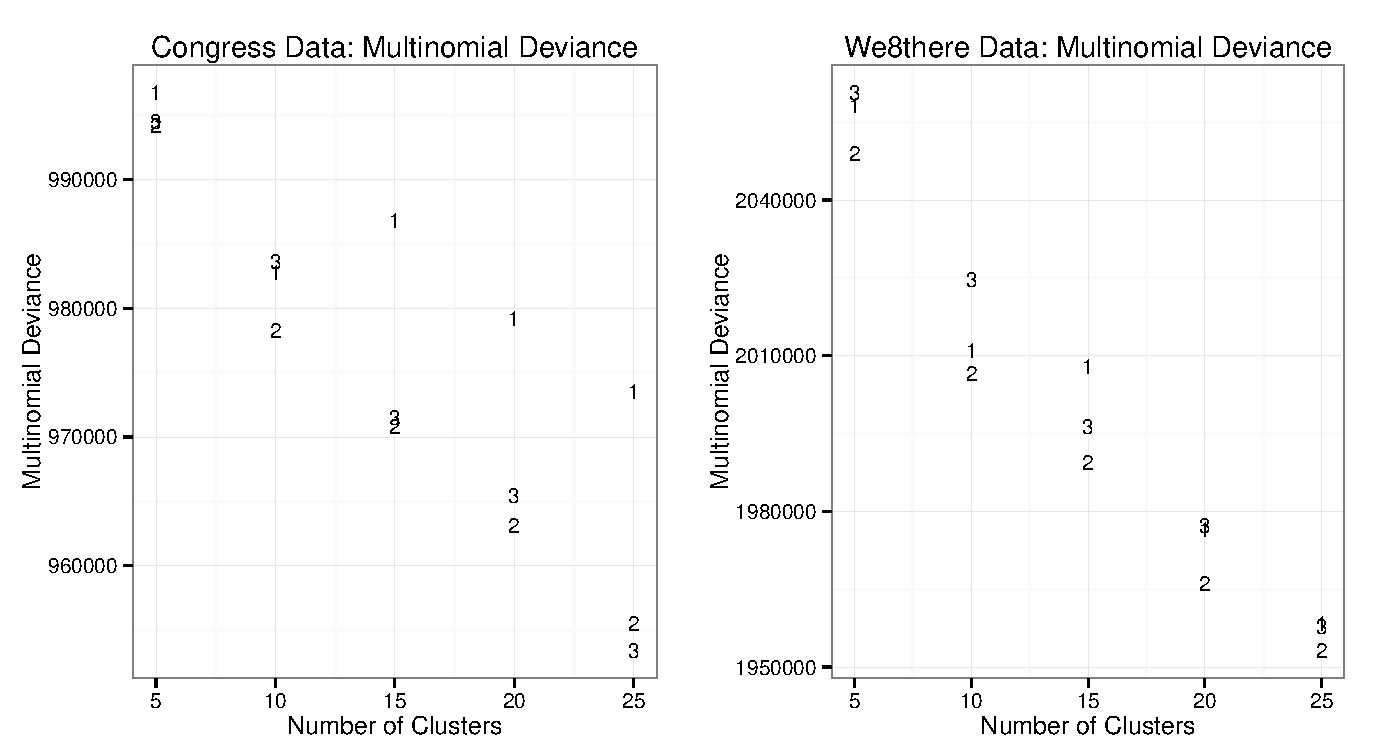
\includegraphics[width=6.2in]{Images/mdev_both.pdf}
  \caption[Multinomial Deviance: Congress Data]
   {Multinomial Deviance from fitted model cluster membership model}
\floatfoot{1 : random cluster initialization, 2 : K Means, 3 : K means on residuals}
\end{figure}


We note that, for any given number of clusters, a better-fitting model is almost always obtained by initializing the cluster memberships on the text data, compared to assigning each document to a random cluster.
We also note that initializing the cluster memberships to the residuals of the text data regressed on the outcome variable (in this case, GOP party membership) usually produced a worse-fitting model than simply initializing membership on the original text data.


Previous research (Taddy 2012) has shown that the optimal number of topics for a topic model on this dataset is around 10. This fact is not shown in our data for a couple of reasons.  First, the cluster membership model is much less flexible than a standard topic model, and would likely need many more clusters to model the same lexical variation. Second, we are possibly over-fitting the data, since these models are not run under cross-validation.

%Do this later dog. 1
%\subsection{Evaluation of Cluster Initialization} 
%Possibly remove
%Method 2: \\
%Clustering the congressional members by speech content led to the overwhelming (majority around 450) being placed in the same cluster, with 1, 3, and 74 persons in the other clusters. After running the algorithm, clusters seemed to be more or less random
%\\
%Method 3:\\
%Clustering the congressional members by unexplained speech content (that is, on the residuls of the regression of party affiliation led to similar results, albiet that the size of the main cluster increased from 450 to 500 congressional members. 
%After the algorithm, 

%\subsection{Convergence and Stability of Clusters}

%textbf{Possibly remove}
%Of key interest is knowing whether or not the algorithm converges to the same clusters when run repeatedly on the same data, and also how this convergence is affected by the 3 proposed cluster initialization.

\subsection{Interpretation of Topics}

An essential aspect of topic modeling is determining the overall theme from the loadings vector. Previous research shows that correctly-specified topic models allow for rich interpretation of themes that can change over time, as well as model relationships between themes (Blei and Lafferty, 2006, and Blei and Lafferty, 2006b). 

Of particular importance in our model is that our extreme simplification of topic weights does impede the ability to discover common themes across documents.
If the topics produced by our method bear no relation to the topics produced by more complex topic modeling approaches, then there is little benefit of our model, regardless of computational improvements and model simplicity. 

To test topic fit, we compare topics produced from our method with the topics produced by fitting a topic-only model, via MAP, with 12 topics on the Congressional Data (Gentzkow and Shapiro, 2010). Fortunately, we find that topics from our model are, in many cases, similar to topics obtained by traditional methods. As an example, table 4 shows a "stem cell" topic found by our method, compared to a similar topic found using the topic-only model mentioned above. The table consists of, for both models, the words with the highest loadings, or weight, in that topic, in decreasing order. This is equivalent to a list of the words with the highest components of cluster coefficient $\Gamma_j$.

\begin{table}[!htbp]
\begin{threeparttable}
\caption{Comparison of top word loadings on a stem-cell topic} \label{tab:title}
\centering
\begin{tabular}{  c  c }
Cluster Membership & Topic Model (LDA)* \\
\hline
umbilic.cord.blood & pluripotent.stem.cel \\
cord.blood.stem  & national.ad.campaign \\
blood.stem.cel   & cel.stem.cel \\
adult.stem.cel & stem.cel.line \\
\end{tabular}
\begin{tablenotes}
\small
\item  *Results reported in Taddy (2012)
\end{tablenotes}
\end{threeparttable}
\end{table}

\subsection{Interpretation of results}

We first evaluate our model by comparing the coefficients predicting GOP to a gamma lasso regression without any topic models. 
The words with the highest loading for determining party affiliation are illustrated in Table 4. This is equivalent to the list of words with the highest components in $\beta$.
We see that some phrases have high loadings on GOP affiliation for both models, like `weapon grade plutonium' and `speaker table' (A stemmed version of `Speaker of the table'). These are words that are, on general, used by many Republicans. 
Phrases such as `People Middle East', which appears in the model without cluster memberships but is not as strongly indicative of GOP affiliation once cluster topics are added, are evidence that some terms are better explained by a particular topic than by party affiliation as a whole. 
Finally, we note that the coefficients in Table 4 are higher for the Cluster Membership model than for the multinomial model without clusters. This is because the addition of clusters to the model allows more flexible modeling that enables a closer fit. In this sense, too many clusters will cause over-fitting. General guidelines on the number of topics to be included in a model are well-documented by Taddy (2012).


% latex table generated in R 3.0.2 by xtable 1.7-1 package
% Sat May 03 15:01:23 2014
\begin{table}[!htbp]
\begin{threeparttable}
\caption{Words with highest loadings for predicting Republican-party affiliation}
\centering
\begin{tabular}{r l l | l  l }
 & \multicolumn{2}{c}{Cluster Membership*} &  \multicolumn{2}{c}{Multinomial Regression}  \\
  \hline
 & term & loading & term & loading \\ 
  \hline
1 & ready.mixed.concrete & 9.25 & un.official & 5.47 \\ 
  2 & driver.education & 7.34 & people.middle.east & 5.47 \\ 
  3 & speaker.table & 7.2 & speaker.table & 5.47 \\ 
  4 & medic.liability.reform & 6.85 & term.care.insurance & 5.47 \\ 
  5 & near.retirement.age & 6.42 & weapon.grade.plutonium & 5.46 \\ 
  6 & weapon.grade.plutonium & 6.23 & national.homeownership.month & 5.46 \\ 
  7 & death.tax.repeal & 5.98 & nation.oil.food & 5.45 \\ 
  8 & commonly.prescribed.drug & 5.72 & united.nation.oil & 5.45 \\ 
  9 & national.ad.campaign & 5.69 & national.heritage.corridor & 5.44 \\ 
  10 & national.homeownership.month & 5.37 & feder.air.marshal & 5.42 \\ 
\end{tabular}
\begin{tablenotes}
\small
\item *Mixed model fit with 15 topics, each topic initialized with K-means on the word count matrix
\end{tablenotes}
\end{threeparttable}
\end{table}


The theory behind our mixed topic model regression predicts that the topics should be able to incorporate a specific theme important to a group of individuals, leaving behind the more general predictors of party-affiliation to the regression coeffecient.
We can test this prediction by examining terms that are significant for a Multinomial Regression without topics, but decrease in importance once topic models are added. For a simple illustration, we choose the phrase "nation oil food", which predicts affiliation with the Republican party.  The term is strongly associated with a topic we might call "domestic issues" topics, whose most likely words are displayed in Table 5.

%We find that these terms are now associated with specific topics and specific groups of politicians, instead of being confounded with general party-affiliation.




% latex table generated in R 3.0.2 by xtable 1.7-1 package
% Wed May 07 18:31:04 2014
\begin{table}[ht]
\centering
\begin{threeparttable}
\caption{Top word loadings of the "domestic issues" topic (Congress data)}
\begin{tabular}{rll}
  \hline
 & term & loading \\ 
  \hline
1 & nation.oil.food & 20.09 \\ 
  2 & united.nation.oil & 12.09 \\ 
  3 & liberty.pursuit.happiness & 8.11 \\ 
  4 & life.liberty.pursuit & 8.11 \\ 
  5 & minority.women.owned & 6.73 \\ 
  6 & universal.health & 6.67 \\ 
  7 & white.care.act & 6.64 \\ 
  8 & ryan.white.care & 6.6 \\ 
  9 & universal.health.care & 5.99 \\ 
  10 & growth.job.creation & 5.39 \\ 
  11 & drilling.arctic.national & 5.3 \\ 
  12 & tax.relief.package & 5.29 \\ 
  13 & judge.john.robert & 5.26 \\ 
  14 & fre.enterprise & 5.07 \\ 
  15 & arctic.refuge & 4.93 \\ 
   \hline
\end{tabular}
\begin{tablenotes}
\small
\item One cluster from a model fit with 20-clusters, each having been initialized with K-means on the residuals of metadata regression
\end{tablenotes}
\end{threeparttable}
\end{table}


We also notice that the members of this cluster (by our simplification, each observation can only be a member of one topic) are 3 Republicans and 8 Democrats. 
The ability to group observations that may have different metadata (in this case, political party) is a benefit of our mixed regression-topic model approach. 
Under standard multinomial regression, observations cannot be grouped by topics.

\subsection{Comparison to Blei's Inverse Regression Topic Model}
As mentioned in Rabinovich and Blei (2014), the addition of latent topics to a model of text data with attributes is the ability to gain an intuitive concept to how metadata affects the distribution of a given topic. 
To demonstrate this effect, we use the graphical model presented in the Rabinovich and Blei paper to show the Democrat/GOP distortion to the `domestic issues'  topic shown mentioned previously. 

The algorithm detected a cluster of words, commonly mentioned together, and the graph shows, on the left panel, this cluster as used by Democrats, in order from most used (top) to less used (bottom). On the right panel, the same cluster is distorted by the coefficient for Republican-party affiliation, where the value of the coefficient is displayed by the horizontal position of the word. Like the left panel, the vertical ordering of the words depicts the most used (top) to less used (bottom) words, and we see that the order has changed for some words that have a strong Republican connotation. For example, Republicans are much more likely to mention the noun phrases `un official' or `death tax repeal'. 

\begin{figure}[!htpb]
  \centering
\caption[Loadings]{Congress 109: Cluster word loadings with covariate distortion}
  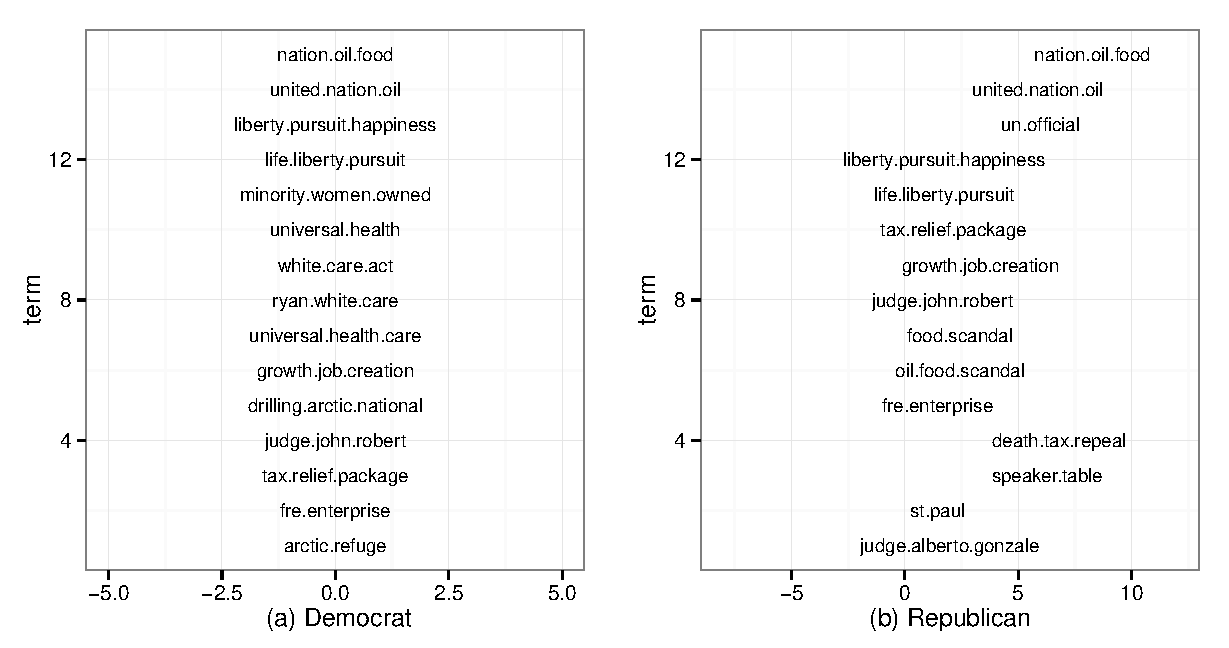
\includegraphics[width=6.2in]{Images/Blei_Changing_Loadings_GOP.pdf}
\floatfoot{A cluster from the Congressional data. On the left are, from highest (top) to lowest (bottom) , terms with the largest Democratic word loadings. On the right are the words with the highest Republican word loadings, also sorted. The horizontal position indicates the value of $\phi$, or distortion on word distribution predicted by being a Republican.}
\end{figure}


\subsection{Restaurant Reviews: We8there Data}

We briefly illustrate the results of the cluster membership model on the we8there corpus of restaurant reviews with a table of word loadings for a selected cluster, as well as a distortion graph of that topic. 
As with the Congress data, we note that despite the simplicity of our model, we obtain meaningful clusters. Table 6 illustrates a cluster we might label as `pizza diner'. 


% latex table generated in R 3.0.2 by xtable 1.7-1 package
% Fri May 09 11:56:25 2014
\begin{table}[ht]
\centering
\begin{threeparttable}
\caption{Top word loadings of the "pizza diner" topic (we8there data)}
\begin{tabular}{rll}
  \hline
 & term & loading \\ 
  \hline
1 & deep dish & 7.76 \\ 
  2 & italian beef & 7.07 \\ 
  3 & pizza like & 6.85 \\ 
  4 & style food & 6.69 \\ 
  5 & au jus & 6.33 \\ 
  6 & cut fri & 6.16 \\ 
  7 & just ok & 6.01 \\ 
  8 & great pizza & 5.96 \\ 
  9 & south side & 5.94 \\ 
  10 & pizza great & 5.82 \\ 
  11 & just over & 5.75 \\ 
  12 & took seat & 5.72 \\ 
  13 & golden brown & 5.61 \\ 
  14 & behind counter & 5.58 \\ 
  15 & got littl & 5.52 \\ 
   \hline
\end{tabular}
\begin{tablenotes}
\small
\item One cluster from a model fit with 15 clusters , each having been initialized with K-means on the original text
\end{tablenotes}
\end{threeparttable}
\end{table}


As with the Congressional data, we also show the effect of metadata regression on the topic weights. However, the analysis for the food reviews data is different from the congressional data: instead of a binary response for party affiliation, the covariate in the we8there data is the overall food review score, from 1 (low) to 5 (high). Phrases with high $\beta$ coefficients are predictive of a higher review score.

\begin{figure}[!htpb]
  \centering
\caption[Loadings]{we8there: Cluster word loadings with and without  metadata distortion}
  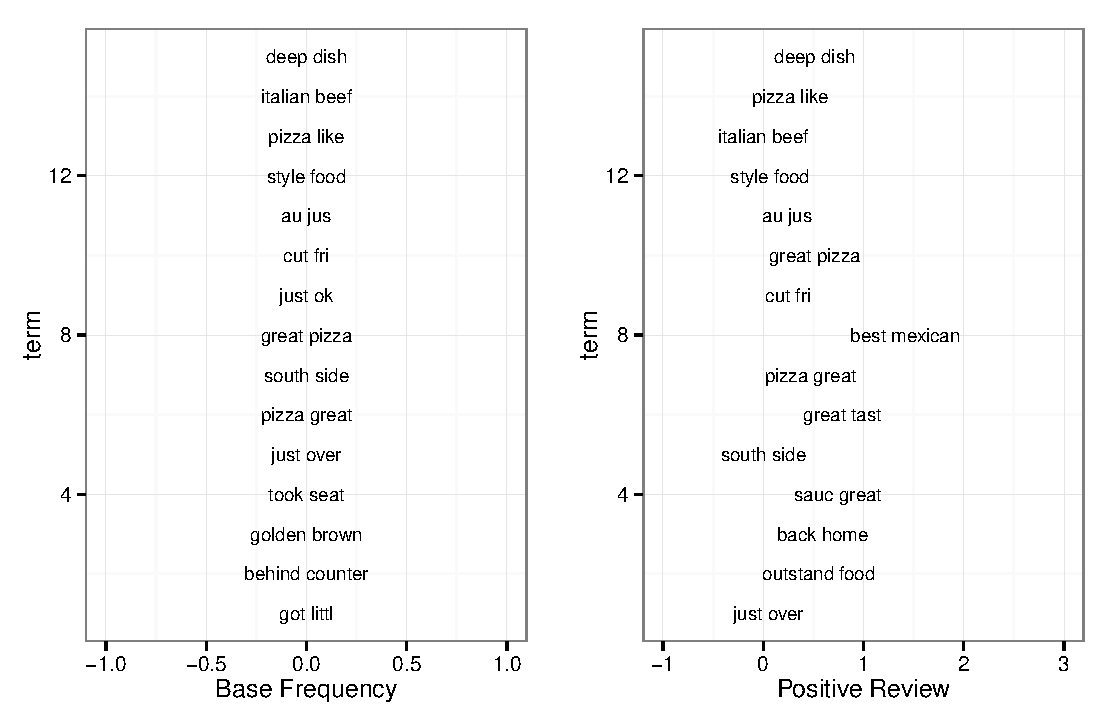
\includegraphics[width=6.2in]{Images/we8there_distortion.pdf}
\floatfoot{A cluster from the we8there restaurant reviews dataset. On the left are, from highest (top) to lowest (bottom), terms with the largest word loadings in this given cluster. On the right are the word loadings of the cluster altered by a positive review. The horizontal position indicates the value of $\phi$, or distortion on word distribution predicted by a positive review.}
\end{figure}

A brief interpretation of the results is as follows: The algorithm grouped the documents into clusters, one of which is characterized by high usage of the words displayed on the left panel of Figure 3. This fitted cluster is not related to the restaurant rating. However, we can visualize what a highly positive review of the food in the cluster might look like by adding the rating coefficient, which we do on the right panel. The change in vertical ordering from the left panel to the right shows how the most common words we would expect to see changes when the review is positive, while the horizontal position shows the weight of each word's coefficient on a review being positive. Preprocessing of the data makes it less easy to reconstruct the exact phrases, but we can see that the phrases `pizza great' (originally `pizza is/was great'), `great taste', and `deep dish' are associated with positive reviews. 

The presence of the term `best mexican' in the `pizza diner' cluster distorted by a positive review illustrates one fundamental drawback of our model. Because we do not model relationship between cluster word loadings and covariate distortion word loadings, combining the two will predict collections of terms that may never appear together in the actual data. The shortcoming is also mentioned in other work on text analysis and metadata (Rabinovich and Blei, 2014), and possible solutions will be mentioned in the next section.


\section{Extension}\label{extensions}

\subsection{Feature Allocations}
A promising extension of the cluster membership model is the generalized `feature allocation' (Broderick et al. 2013), where each observation can be attributed multiple features. This setup is an intermediary between our cluster membership model and a traditional topic model. 
The algorithm provided in this paper could be extended to incorporate a feature allocation, although the order of step 3 of the algorithm increases from linear $\mathcal{O}_{cluster} = n_k$ to $\mathcal{O}_{feature} = 2^{n_k}$, where $n_k$ refers to the number of clusters/features in the model. This increase in complexity may be reduced through changes to the algorithm, and the model would still enjoy the ability to collapse observations across unique features. 

\subsection{Cross Validation and Prediction}
One drawback of our model is that, in order to train cluster membership, the values of the metadata are required (see algorithm pseudocode in previous section). This hinders the ability to use the method for prediction (where, presumably, we hope to predict missing metadata from the text), and impeded our ability to perform cross validation. One possible solution would be to use k-nearest neighbors or other appropriate algorithm to assign each document of the test data to a cluster, after fitting a model with training data. However, this approach would be difficult to combine with the feature allocation extension proposed above, since the $n$ observations would be separated into $2^{n_k}$ partitions, instead of $n_k$. 

\subsection{Modeling relationships between clusters and metadata}
As noted in a previous section, one drawback of our model is the lack of relationship between clusters and metadata distortion vectors. 
Previous work on topic models allowed for correlation between topics (Blei \& Lafferty 2006) and has successfully applied these models to complicated datasets (Blei \& Lafferty 2007).
Other authors have noted this problem (Rabinovich \& Blei 2014), and possible solutions include allowing a range of metadata distortion vectors with varying relationships to each cluster or topic. 


\section{Conclusion}\label{conclusion}

In this paper, we have reviewed the theory behind topic modeling and regression on metadata in text data. 
We introduce an algorithm that combines the metadata regression techniques developed by Taddy (2013a, 2013b) with a simple adaptation of the classic topic model.
We then applied our algorithm to two large, sparse text datasets and report the results, noting that the simple cluster membership is able to identify similar topics found in more complex LDA models. 
We conclude by suggesting possible extensions of our approach to assist with generalizing and comparing the cluster membership model to alternative models for topic and metadata analysis. 


\section{Acknowledgements}\label{conclusion}

I thank Professor Matt Taddy for his guidance throughout the research and writing of this paper. I also thank Professor Stephen Stigler for his comments paper feedback, the University of Chicago Research Computing Center (RCC) for computational resources, and Eric Janofsky for the helpful discussion. 


\newpage

%\begin{appendix}
%\section{Appendix}

%\vspace{4mm}\noindent 
%The following may be included in an appendix:

%\begin{itemize}
%\item[] Data 
%\item[] Simulation codes
%\item[] Certain derivations
%\end{itemize}
%\end{appendix}
%\newpage

\begin{thebibliography}{99}

\bibitem{Time} Belsky, G. (2012). Why Text Mining May Be The Next Big Thing. Time Magazine, http://business.time.com/2012/03/20/why-text-mining-may-be-the-next-big-thing/

\bibitem{LDA} Blei, D. , Ng, A., and Jordan, M. (2003). Latent Dirichlet allocation. Journal of Machine Learning Research (JMLR), 3:993–1022, March 2003. ISSN 1532-4435

\bibitem{CTM} Blei, D. and Lafferty, J. (2006). Correlated topic models. Advances in Neural Information Processing Systems 18. MIT Press, Cambridge, MA.

\bibitem{Dynamic Topic Models} Blei, D. and Lafferty, J.(2006b). Dynamic Topic Models. Computer Science Department Paper 1038.

\bibitem{CTM Science}  Blei, D. and Lafferty, J. (2007). A Correlated Topic Model of Science. The Annals of Applied Statistics

\bibitem{Paintboxes} Broderick, T.,  Pitman, J.,  and Jordan, M. (2013). Feature allocations, probability functions, and paintboxes. Bayesian Analysis, to appear. Preprint arXiv:1301.6647, 2013

\bibitem{Slant} Gentzkow, M., and  Shapiro, J. What Drives Media Slant? Evidence from U.S. Daily Newspapers. Econometrica, Vol. 78, No. 1 (January, 2010), 35–71

\bibitem{PartialInverseRegression}  Li, Cook  and Tsai. Partial Inverse Regression. Biometrika (2007), 94, 3, pp. 615–625

\bibitem{Porter} Porter, M. (1980). An algorithm for suffix stripping, Program, 14(3) pp 130 - 137.

\bibitem{TopicModelsTaddy} Taddy, M. (2012).On Estimation and Selection for Topic Models.  Proceedings of the 15th International Conference on Artificial Intelligence and Statistics

\bibitem{MNIR} Taddy, M. (2013a). Multinomial inverse regression for text analysis. Journal of the American Statistical Association 108.

\bibitem{GammaLasso} Taddy, M.  (2013b) The Gamma Lasso. arXiv:1308.5623

\bibitem{TwitterSentiment}  Taddy, M.  (2013c) Measuring Political Sentiment on Twitter: Factor Optimal Design for Multinomial Inverse Regression, Technometrics, 55:4, 415-425, DOI

\bibitem{IRTM} Rabinovich, M. and Blei, D. (2014). The Inverse Regression Topic Model. Proceedings of the 31st International Conference on Machine Learning, Beijing, China, 2014. JMLR: W\&CP volume 32







\end{thebibliography}
\end{document}
